\documentclass[10pt,letterpaper]{article}

%\usepackage[latin1]{inputenc} 
\usepackage[utf8]{inputenc}
\usepackage[cyr]{aeguill}
\usepackage[colorlinks=true]{hyperref}
\usepackage{textpos}
\usepackage{graphicx}
\usepackage[french]{babel}
\usepackage{color}
\usepackage{array}
\usepackage{enumerate}
\usepackage{fancyhdr}
\usepackage{lastpage}
\usepackage{amsmath}
\usepackage{amssymb}
\usepackage{epstopdf}
\usepackage{mathrsfs}
\usepackage{float}
\usepackage{multicol}
\usepackage{caption}
\usepackage{subcaption}
\usepackage{siunitx}
\usepackage{rotating}
\usepackage{adjustbox}
\addto\captionsfrench{\def\tablename{Tableau}}

%-----------------------------------------------------------------%
% Definitions
\newcommand{\session}{Hiver 2022}
\newcommand{\firstauthor}{Yoan \textbf{Fournier}}
\newcommand{\firstregistrationnumber}{1958736}
\newcommand{\secondauthor}{Victor \textbf{Gaudreau-Blouin}}
\newcommand{\secondregistrationnumber}{1958297}
\newcommand{\reportnumber}{}
\newcommand{\firsttitle}{Analyse énergétique d'un processeur vectoriel pour des calculs de DNN}
\newcommand{\secondtitle}{Rapport final}
%-----------------------------------------------------------------%



\oddsidemargin 0pt
\topmargin 0pt
\textwidth 6.5in
\textheight 8.1in

\setlength{\parskip}{1em}

\definecolor{bleu_poly}{RGB}{65,170,230}
\definecolor{vert_poly}{RGB}{140,200,60}
\definecolor{orange_poly}{RGB}{250,150,30}
\definecolor{rouge_poly}{RGB}{185,30,50}
\definecolor{gris_poly}{RGB}{166,168,171}


\title{\vspace{-2.5cm} \noindent\makebox[\linewidth]{\color{rouge_poly}{\rule{\textwidth}{1.5pt}}}
        \begin{center}
        \begin{tabular}{m{6.5cm}m{6cm}}
        \textbf{ \huge Projet \reportnumber}  & 
\includegraphics[width=0.4\textwidth]{Polytechnique_signature-CMYK-droite_FR.eps}
        \end{tabular}
        \end{center}
        \noindent\makebox[\linewidth]{\color{rouge_poly}{\rule{\textwidth}{1.5pt}}}
        \\ \  \\
        \Huge \firsttitle \\ \secondtitle  
        \\ \ \\
        \LARGE ELE6307 - Machines neuronales : architectures et applications
        }

\author{\session \\ Département de génie électrique \\ École Polytechnique de Montréal} 

\date{Dernière mise à jour: \today}

\pagestyle{fancy}

\lfoot{\session}
\cfoot{ELE6307 - Machines neuronales : architectures et applications}
\rfoot{\thepage/\pageref{LastPage}}
\chead{}
\lhead{\emph{Projet -- \firstauthor  \, (\firstregistrationnumber)/\secondauthor\,  (\secondregistrationnumber)}}
\rhead{
\includegraphics[width=2.5cm]{Polytechnique_signature-CMYK-droite_FR.eps}}
\renewcommand{\headrulewidth}{0.4pt}
\renewcommand{\footrulewidth}{0.4pt} 
\setlength{\headheight}{45pt}


\graphicspath{{fig/}}


\newcommand{\vb}[1]{\mathbf{#1}}
\newcommand{\bs}[1]{\boldsymbol{#1}}


%-----------------------------------------------------------------%
% SOF
\begin{document}
\maketitle
\noindent\makebox[\linewidth]{\color{rouge_poly}{\rule{\textwidth}{1.5pt}}} 


\noindent \LARGE \firstauthor  \hfill \firstregistrationnumber


\noindent \LARGE \secondauthor \hfill \secondregistrationnumber


\noindent\makebox[\linewidth]{\color{rouge_poly}{\rule{\textwidth}{1.5pt}}}


\newpage
\normalsize



{\bibliography{refs}}
    \bibliographystyle{abbrv}

\section{Introduction}
    \begin{multicols}{2}
    Dans les dernières années, l'utilisation de réseaux de neurones profonds (DNN) pour
    résoudre différentes tâches a beaucoup augmenté. Ces DNNs nécessitent des puissances
    de calculs considérables, mais à la fois nécessitent une bonne efficacité énergétique 
    étant donné leur déploiement dans des appareils mobiles. Bien que les processeurs 
    généralistes que l'on retrouve aujourd'hui ont augmenté rapidement en performance,
    les limitations du \textit{Dennard Scaling} se font ressentir. Il est donc souhaitable
    de trouver une autre approche pour accélérer de façon efficace les calculs dans les DNNs.
    Une manière intéressante pour l'accélération des calculs pour des DNNs est l'utilisation
    de processeurs vectoriels plutôt que des processeurs scalaires standards. Ces processeurs
    utilisent un jeu d'instruction SIMD (\textit{Single instruction, Multiple Data}) plutôt 
    que SISD (\textit{Single instruction, Single data}). Ainsi une instruction SIMD peut
    performer la même opération sur plusieurs données plutôt qu'une seule, ce qui permet 
    de plus facilement augmenter le parallélisme des calculs. 
    
    Le présent rappot étudie l'efficacité énergétique d'un modèle simplifié du processeur
    vectoriel ARA sur différents problèmes en utilisant le simulateur \textit{Timeloop-Accelergy}.
    \end{multicols}

\section{Méthodologie}
    \begin{multicols}{2}

    %TODO: Ajouter paragraphe sur ARA
    L'architecture sur laquelle notre modèle se base est sur celle du coprocesseur 
    vectoriel ARA \cite{ara_paper}. Ce coprocesseur est une extension vectorielle du processeur scalaire
    RISCV CVA6. Le fonctionnement d’ARA se base sur le concept de \textit{Lanes}. 
    La figure \ref{fig:ara_arch} présente l'architecture d’ARA \cite{bougenot_2020}.
    Le coprocesseur ARA possède un nombre d'allées, ou \textit{Lanes}, qui sont capables de traiter des
    éléments vectoriels indépendament. Le routage des données vers ces \textit{Lanes} grandit évidemment en complexité
    avec le nombre de \textit{Lanes}. Le \textit{Sequencer} s'occupe de lire les instructions à exécuter 
    et transmettre les informations correctes au \textit{Vector Load and Store Unit} (VLSU), 
    \textit{Slide Unit} (SLDU) ou aux \textit{Lanes}. Le VLSU est responsable de générer les bonnes
    addresses, amenant les données séquentiellement vers et depuis les \textit{Lanes}. 
    Le SLDU exécute des opérations qui n'ont pas d'indépendance entre les \textit{Lanes}.
    Finalement, chaque \textit{Lane} a son propre \textit{sequencer} pour les instructions à exécuter
    sur son élément vectoriel. Le reste de la \textit{Lane} peut être considéré comme un PE, avec sa mémoire locale,
    un étage de conversion et un étage d'exécution.

    Afin de modéliser l'efficacité énergétique du coprocesseur vectoriel ARA, le simulateur Timeloop a été 
    utilisé. Ce simulateur utilise une structure hiérarchique pour modéliser une architecture. Une structure
    détaillant le problème à résoudre par l'architecture est aussi spécifiée. La commande \textit{timeloop-mapper}
    permet ensuite de trouver automatiquement la correspondance idéale du problème sur l'architecture matérielle.

    {\centering
    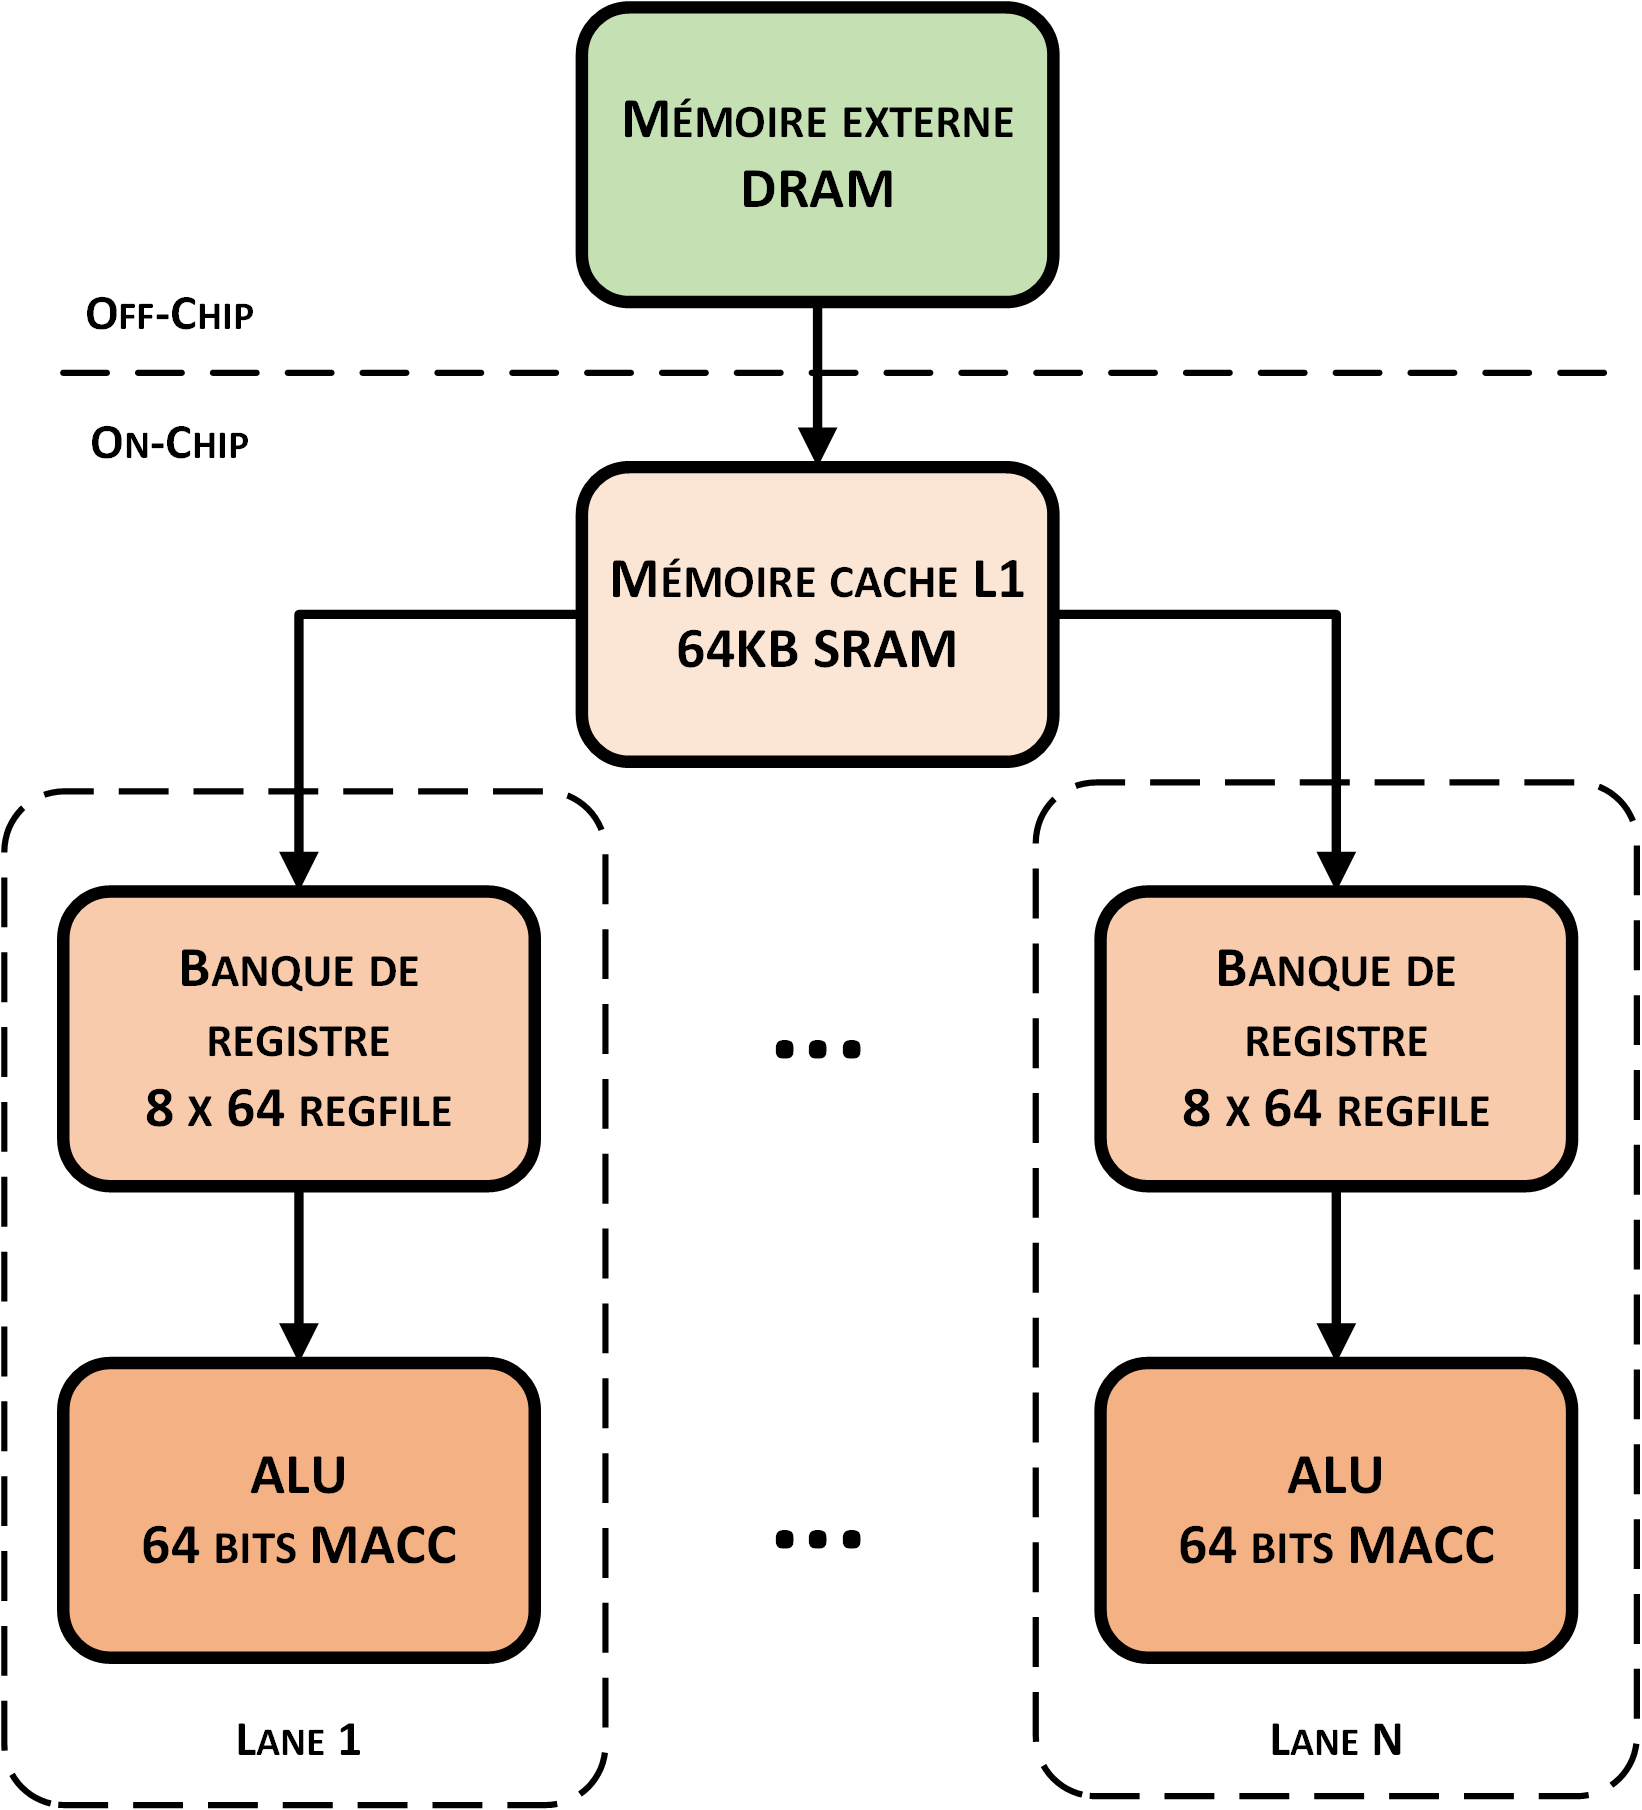
\includegraphics[width=0.8\linewidth]{arch_visio.png}
    \captionof{figure}{Architecture de ARA sur Timeloop}
    \label{fig:arch}}
    \bigskip

    L'architecture simplifiée de ARA, comme mentionnée dans la proposition du projet, peut se modéliser en termes de 
    \textit{Lanes}. Chaque \textit{Lanes} à sa plus simple expression consiste en une banque de 8 registres ainsi qu'une
    unité arithmétique capable d'effectuer des multiplications et des additions. Bien que sur ARA, l'unité d'addition 
    est séparée de l'unité de multiplication, les deux unités peuvent fonctionner durant le même cycle sur des données
    indépendantes. Dans le cadre de la modélisation, on simplifie en utilisant la structure \textit{intmac} fournie par
    l'outil Timeloop-Accelergy. Nous considérons que la différence causée par cette simplification est minimale. En effet,
    les opérations dans une Lane sont pipelinées et les opérations de multiplication et addition peuvent être exécutées en même temps.
    La seule différence principale est la latence causée par le pipelinage des opérations. Cependant, ce n'est pas une métrique
    de performance étudiée dans le cadre de ce projet.

    L'architecture utilisée est présentée à la figure \ref{fig:arch}. On y observe une mémoire DRAM principale reliée à 
    la mémoire cache L1 de 64 KB. La cache L1 est reliée à un nombre paramétrable de \textit{Lanes}. 
    Chaque \textit{Lane} comporte sa banque de 8 registres et son unité de \textit{multiply-accumulate}.

    %TODO: Changer ce paragraphe
    Afin d'étudier la performance de l'architecture en fonction du nombre de \textit{Lanes}, le problème utilisé est la première 
    couche convolutionnelle du modèle VGG16. Cette couche comporte 64 filtres avec un \textit{kernel} de $3\times3$. L'entrée de la couche
    est une image de dimension $224\times224\times3$.  

    \end{multicols}

\section{Résultats}
    \begin{multicols}{2}
        
    {\centering
    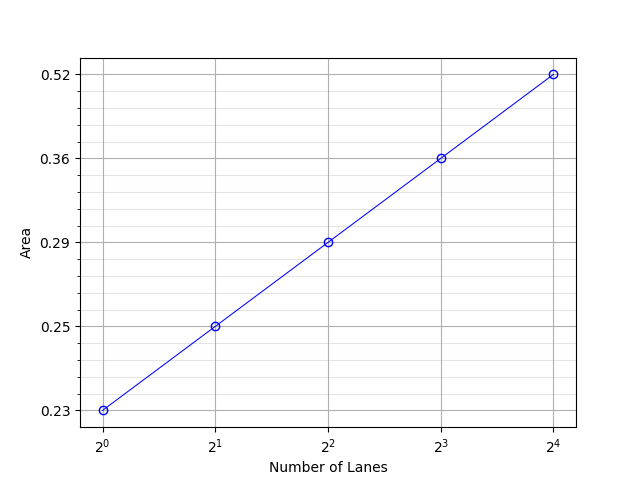
\includegraphics[width=\linewidth]{area.png}
    \captionof{figure}{Aire de ARA en fonction du nombre de \textit{Lanes}}
    \label{fig:area}}
    \bigskip

    {\centering
    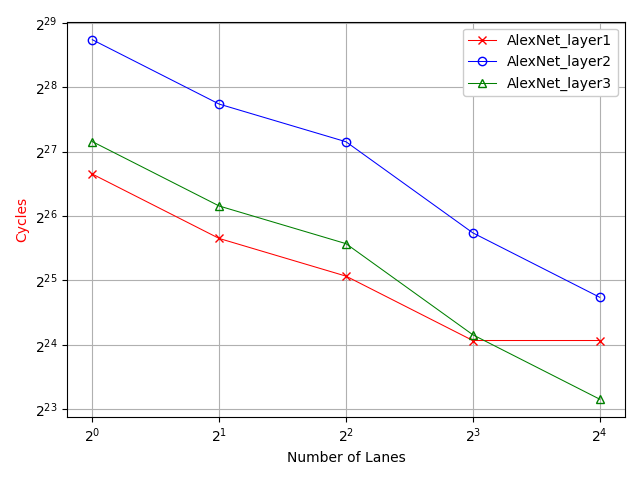
\includegraphics[width=\linewidth]{Alex_cycles.png}
    \captionof{figure}{Cycles de ARA en fonction du nombre de \textit{Lanes} pour le problème AlexNet}
    \label{fig:cycles_alex}}
    \bigskip

    {\centering
    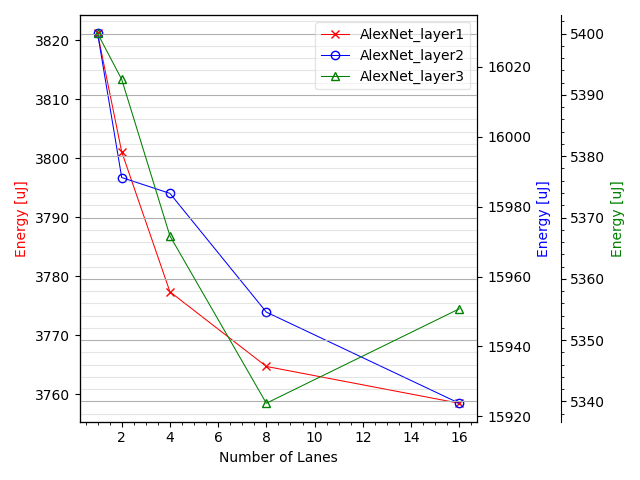
\includegraphics[width=\linewidth]{Alex_energy.png}
    \captionof{figure}{Cycles de ARA en fonction du nombre de \textit{Lanes} pour le problème AlexNet}
    \label{fig:energy_alex}}
    \bigskip

    {\centering
    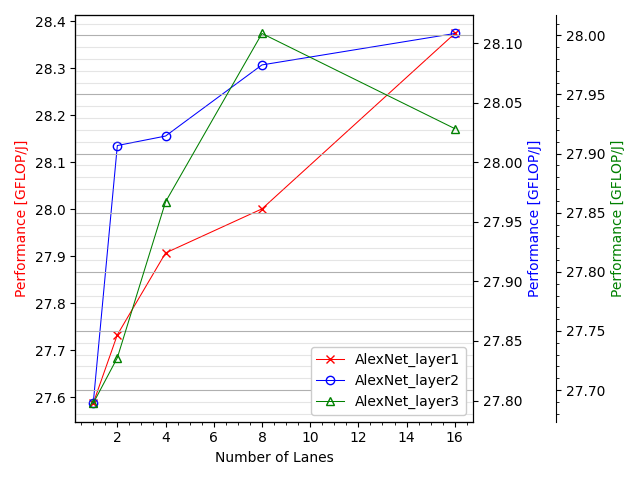
\includegraphics[width=\linewidth]{Alex_performance.png}
    \captionof{figure}{Cycles de ARA en fonction du nombre de \textit{Lanes} pour le problème AlexNet}
    \label{fig:perf_alex}}
    \bigskip

    {\centering
    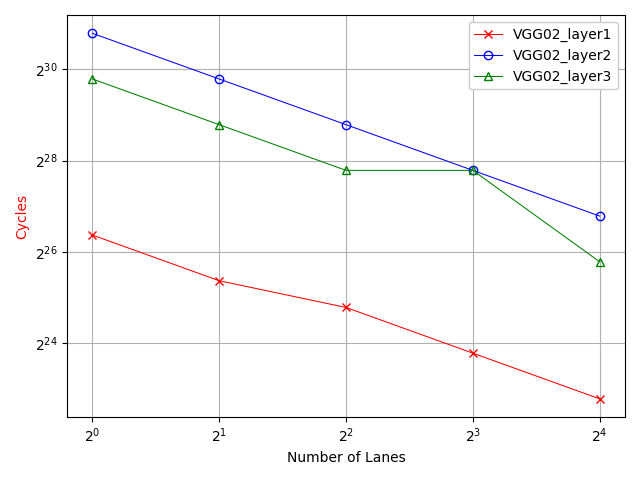
\includegraphics[width=\linewidth]{VGG_cycles.png}
    \captionof{figure}{Cycles de ARA en fonction du nombre de \textit{Lanes} pour le problème VGG16}
    \label{fig:cycles_vgg}}
    \bigskip

    {\centering
    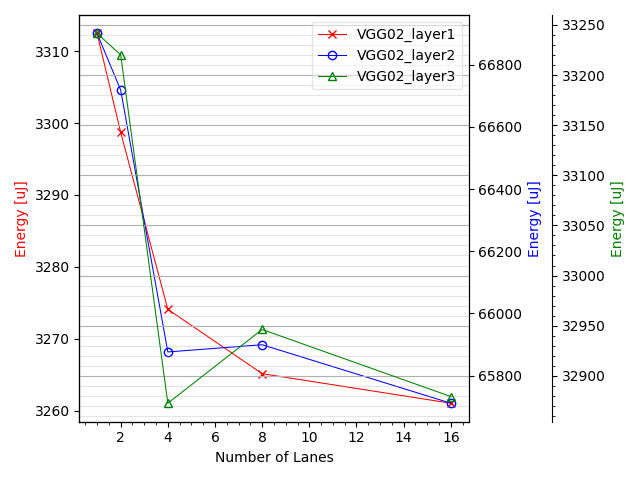
\includegraphics[width=\linewidth]{VGG_energy.png}
    \captionof{figure}{Cycles de ARA en fonction du nombre de \textit{Lanes} pour le problème VGG16}
    \label{fig:energy_vgg}}
    \bigskip

    {\centering
    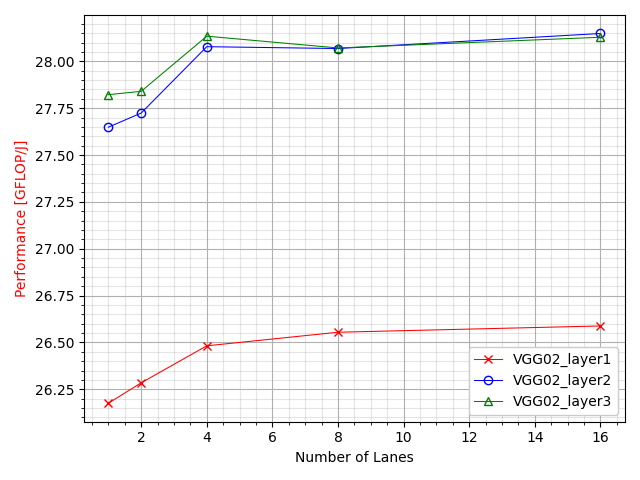
\includegraphics[width=\linewidth]{VGG_performance.png}
    \captionof{figure}{Cycles de ARA en fonction du nombre de \textit{Lanes} pour le problème VGG16}
    \label{fig:perf_vgg}}
    \bigskip

    \begin{table}[H]
        \centering
        \begin{tabular}{l|cc}
        Problem                     & \multicolumn{2}{c}{\textbf{AlexNet\_layer2}}                                           \\
        Parameters                  & \multicolumn{2}{c}{\begin{tabular}[c]{@{}c@{}}M=256 K=5x5\\ C=96 I=27x27\end{tabular}} \\
        n                           & \multicolumn{2}{c}{16}                                                                 \\
        Mapper                      & \multicolumn{1}{c|}{Timeloop}                         & Custom                         \\ \hline
        Utilization                 & 0.62                                                  & 1                              \\
        Cycles {[}Millions{]}       & 44.8                                                  & 28.0                           \\
        Energy {[}mJ{]}             & 15.92                                                 & 15.90                          \\
        \textbf{Perf {[}GFLOP/J{]}} & 27.90                                                 & 28.18                         
        \end{tabular}
        \caption{Mapping Timeloop et mapping custom pour AlexNet L2}
        \label{fig:alex_L2_custom_map}
    \end{table}    
    \bigskip

    \end{multicols}

\section{Conclusion}

{\bibliography{refs}}
    \bibliographystyle{abbrv}

\pagebreak
    \begin{sidewaystable}[h]
\vspace{-5.7cm}
\centering
\section*{Annexe}
    \bigskip
    \bigskip
    \bigskip
        \footnotesize
        \begin{tabular}{l|ccccc|ccccc|ccccc}
        Problem                     & \multicolumn{5}{c|}{\textbf{AlexNet\_layer1}}                                           & \multicolumn{5}{c|}{\textbf{AlexNet\_layer2}}                                          & \multicolumn{5}{c}{\textbf{AlexNet\_layer3}}                                            \\
        Parameters                  & \multicolumn{5}{c|}{\begin{tabular}[c]{@{}c@{}}M=96 K=11x11\\ C=3 I=55x55\end{tabular}} & \multicolumn{5}{c|}{\begin{tabular}[c]{@{}c@{}}M=256 K=5x5\\ C=96 I=27x27\end{tabular}} & \multicolumn{5}{c}{\begin{tabular}[c]{@{}c@{}}M=384 K=3x3\\ C=256 I=13x13\end{tabular}} \\
        n                           & 1                & 2                & 4               & 8              & 16             & 1                & 2               & 4               & 8              & 16             & 1                & 2                & 4               & 8              & 16             \\ \hline
        Utilization                 & 1                & 1                & 0.75            & 0.75           & 0.94           & 1                & 1               & 0.75            & 1              & 0.62           & 1                & 1                & 0.75            & 1              & 1              \\
        Cycles {[}Millions{]}       & 105.4            & 52.7             & 35.1            & 17.6           & 7.3            & 447.9            & 223.9           & 149.3           & 56.0           & 44.8           & 149.5            & 74.8             & 49.8            & 18.7           & 9.3            \\
        Energy {[}mJ{]}             & 3.82             & 3.80             & 3.77            & 3.77           & 3.76           & 16.03            & 15.99           & 15.98           & 15.95          & 15.92          & 5.40             & 5.39             & 5.36            & 5.34           & 5.35           \\
        \textbf{Perf {[}GFLOP/J{]}} & 27.59            & 27.73            & 27.91           & 28.00          & 28.12          & 27.94            & 28.01           & 28.02           & 28.08          & 27.90          & 27.69            & 27.73            & 27.86           & 28.00          & 27.92         
        \end{tabular}
        \caption{Résultats pour le problème AlexNet}
        \label{fig:results_alex}
        
    \bigskip
    \bigskip
    \bigskip
    \bigskip

        \footnotesize
        \begin{tabular}{l|ccccc|ccccc|ccccc}[
        Problem                     & \multicolumn{5}{c|}{\textbf{VGG02\_layer1}}                                             & \multicolumn{5}{c|}{\textbf{VGG02\_layer2}}                                              & \multicolumn{5}{c}{\textbf{VGG02\_layer3}}                                               \\
        Parameters                  & \multicolumn{5}{c|}{\begin{tabular}[c]{@{}c@{}}M=64 K=3x3\\ C=3 I=224x224\end{tabular}} & \multicolumn{5}{c|}{\begin{tabular}[c]{@{}c@{}}M=64 K=3x3\\ C=64 I=224x224\end{tabular}} & \multicolumn{5}{c}{\begin{tabular}[c]{@{}c@{}}M=128 K=3x3\\ C=64 I=112x112\end{tabular}} \\
        n                           & 1                & 2               & 4               & 8               & 16             & 1                & 2               & 4               & 8               & 16              & 1                & 2               & 4               & 8               & 16              \\ \hline
        Utilization                 & 1                & 1               & 0.75            & 0.75            & 0.75           & 1                & 1               & 1               & 1               & 1               & 1                & 1               & 1               & 0.5             & 1               \\
        Cycles {[}Millions{]}       & 86.7             & 43.4            & 28.9            & 14.5            & 7.2            & 1850             & 924.8           & 462.4           & 231.2           & 115.6           & 925              & 462             & 231             & 231             & 57.8            \\
        Energy {[}mJ{]}             & 3.31             & 3.30            & 3.27            & 3.27            & 3.26           & 66.9             & 66.7            & 65.9            & 65.9            & 65.7            & 33.2             & 33.2            & 32.9            & 32.9            & 32.9            \\
        \textbf{Perf {[}GFLOP/J{]}} & 26.18            & 26.28           & 26.48           & 26.55           & 26.59          & 27.65            & 27.72           & 28.08           & 28.07           & 28.15           & 27.82            & 27.84           & 28.13           & 28.07           & 28.13          
        \end{tabular}
        \caption{Résultats pour le problème VGG16}
        \label{fig:results_vgg}  
    \end{sidewaystable}

\end{document} 
%-----------------------------------------------------------------%
% EOF